\documentclass[tikz]{standalone}


\usepackage{graphicx}
\usepackage{pxfonts}
\newcommand{\figf}{\sffamily\textbf}

\begin{document}
\sffamily

\begin{tikzpicture}[anchor = north west]

	\clip (0,0) rectangle +(18,-9.5);


	\begin{scope}
		\node at (-0.6,0.3){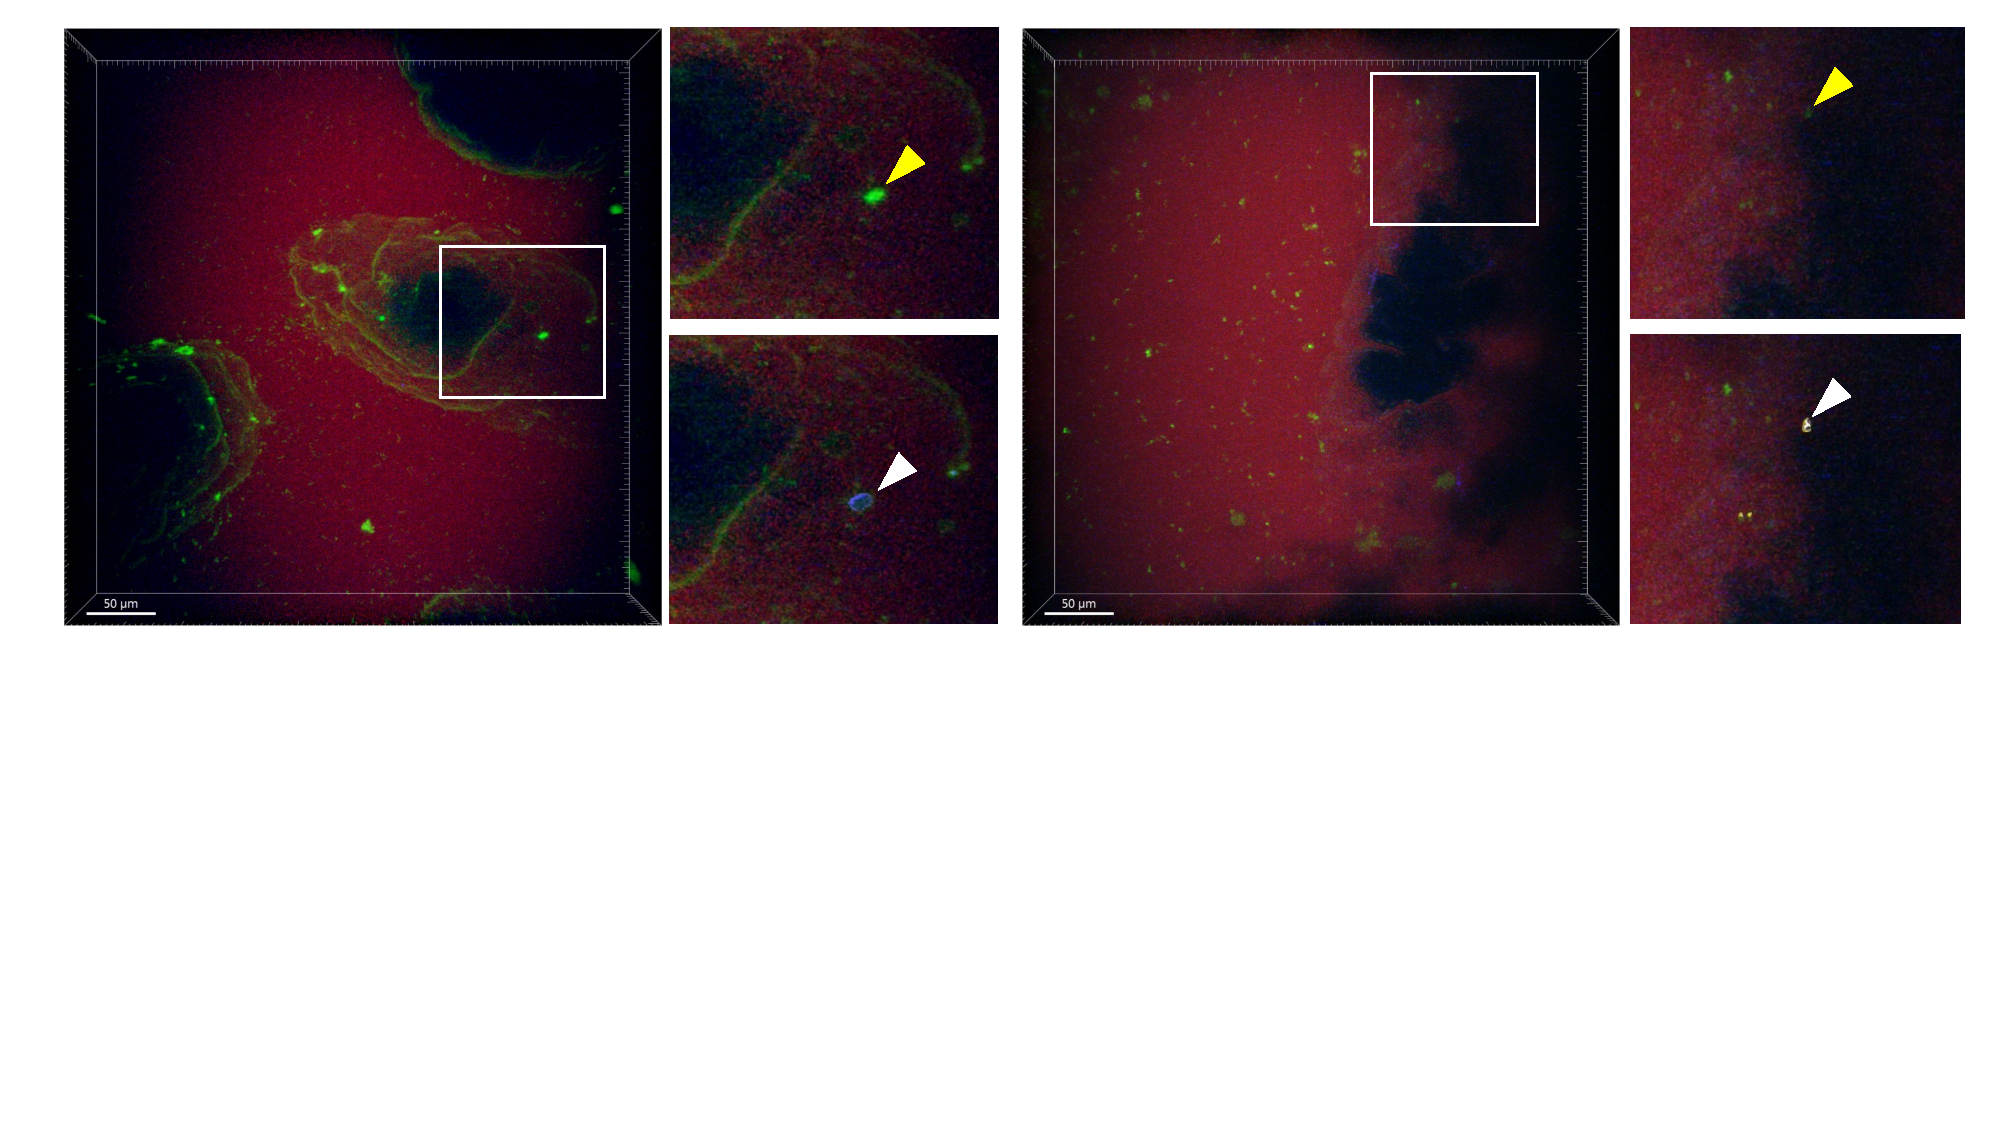
\includegraphics[width=1.1\textwidth]{../img/flaA-mut.pdf}};
		\node[white] at (0,0) {\figf A};
		\node[white] at (6.35,0) {\figf B};
		\node[green] at (0.4,-0.05) {\scriptsize 10403 Lm-RT};
		\node[red] at (0.4,-0.35) {\scriptsize Rh-Dex};
		\node[green] at (6.75,-0.05) {\scriptsize flaA\textsuperscript{mut} Lm-RT};
		\node[red] at (6.75,-0.35) {\scriptsize Rh-Dex};
	\end{scope}

	\begin{scope}[yshift = -4cm ]
		\node at (0.5,-0.5) {\includegraphics{../plots/panelC.pdf}};
		\node at (0,0) {\figf C};
	\end{scope}
	
	\begin{scope}[xshift = 7.25cm, yshift=-4cm]
		\node at (0.4,0) {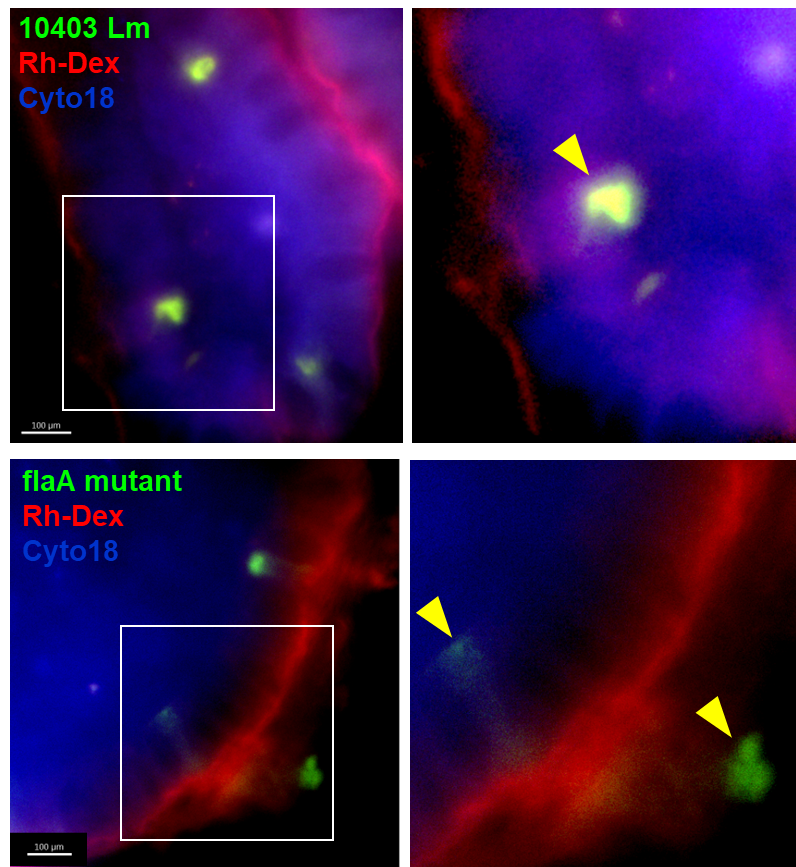
\includegraphics[width=0.4\textwidth]{../img/GC_stain.png}};
		\node at (0,0) {\figf D};
		\node at (0,-2.8) {\figf E};
	\end{scope}

	

\end{tikzpicture}

\end{document}